\documentclass{article}

\usepackage[margin=2.5cm]{geometry}

\usepackage[utf8]{inputenc}
\usepackage[T1]{fontenc}
\usepackage[german]{babel}

\usepackage{hyperref}
\hypersetup{
pdftitle={Pflichtenheft},
bookmarks = true
}
\usepackage[toc]{glossaries}

\usepackage{graphicx}

\usepackage[shortlabels]{enumitem}
\usepackage{parskip}

\usepackage{float}
\floatplacement{figure}{H}
\usepackage{placeins}

\usepackage{amsmath}
\usepackage{amssymb}

%\usepackage{svg}
%\usepackage{algpseudocode}
%\usepackage{algorithm}
\usepackage{caption}
\usepackage{subcaption}
%\usepackage{fancyvrb}
%\usepackage{tgcursor}
%\fvset{frame=single,framesep=1mm,fontfamily=courier,fontsize=\scriptsize,numbers=left,framerule=.3mm,numbersep=1mm,commandchars=\\\{\}}




\usepackage{fix-cm}
\newcommand{\titlesize}{\fontsize{30pt}{20pt}\selectfont}
\newcommand{\themesize}{\fontsize{20pt}{20pt}\selectfont}
\newcommand{\authorsize}{\fontsize{15pt}{20pt}\selectfont}

\newcommand{\mypackage}[1]{\subsection*{Package #1} \label{#1} \addcontentsline{toc}{subsection}{\nameref{#1}}}
\newcommand{\myclass}[1]{\subsubsection*{Class #1} \label{#1} \addcontentsline{toc}{subsubsection}{\nameref{#1}}}
\newcommand{\myinterface}[1]{\subsubsection*{Interface #1} \label{#1} \addcontentsline{toc}{subsubsection}{\nameref{#1}}}

%\makeglossaries



%\titlehead{\centering \includegraphics{images/title}}
%\title{RaGE Pflichtenheft}
%\author{Jonas Kasper, Bernard Hohmann, Thomas Fischer, Christian Jung, Jonas Linßen}

\begin{document}
	%\maketitle
	
	%\newpage
	
	\begin{titlepage}
		%\centering \includegraphics[width=0.7\textwidth]{images/title}
		
		\titlesize \hspace*{.5cm} Random Graph Coloring Evaluation
		~\newline~\newline
		
		\themesize \hspace*{3cm} Entwurfsdokument
		\newline~\newline
		
		\authorsize Jonas Kasper, Bernard Hohmann, Thomas Fischer, Christian Jung, Jonas Linßen
	\end{titlepage}
	
	\tableofcontents
	\newpage
	
	\section{Anmerkungen zum Pflichtenheft}
	\subsection{Klarstellungen}
	\subsection{Änderungen}	
	\subsubsection{GUI}
			%\begin{enumerate}
			\paragraph{Graphen-Vorschau}
				%Worum geht es?
				In der Graph-Preview Ansicht in der GUI werden die einzelnen Graphen, seien sie generiert oder importiert, unter einem neuen Tab angezeigt.
				
				%Wie war es bisher?
				Diese Anzeige war bisher so gestaltet, dass die Graphen in einer Grid-View gesetzt werden.
				Dies würde in einer tabellenartigen Darstellung resultieren, bei der Beispielsweise 2 Spalten und 3 Reihen für die Graphen gleichzeitig dargestellt werden.
				
				%Was war Grund der Änderung:
				Diese Ansicht hatte den Nachteil, dass der User immer gezeichnete Graphen vor sich sieht.
				Dies führt zu deutlich geringerer Übersichtlichkeit.
				Außerdem bestand kein großes Interesse des Kunden daran, dass man die zuvor generierten Graphen sofort betrachten kann.
					Das graphische Darstellen der Graphen wurde eher an anderer Stelle gewünscht.
				Darüber hinaus ist diese Art der Ansicht nicht besonders gut skalierbar, wenn der User die Fenstergröße anpassen möchte, besteht die Gefahr, dass die Graphen-Bilder zu klein werden, um anschaulich zu sein.
				
				%Was ist die Änderung?
				Aus diesem Grund haben wir die Ansicht zu einer Tab-View geändert.
				Dies bedeutet, dass man nun eine Liste an ausklappbaren Tabs mit den jeweiligen Graphen-Namen vor sich sieht.
				Demzufolge kann man bei Interesse die Graphen-Tabs ausklappen.
					Beim Ausklappen wird dann genau dieser zu betrachtende Graph gezeichnet.
					Daraus folgt, dass man nicht mehr mit Graphen-Zeichnungen überschüttet wird.
				
				%Folgen für das weitere Programm
				Durch diese Änderung entsteht ein weiterer Vorteil.
				Die Performance des Programms wird verbessert, da das Programm nicht sofort alle Graphen zeichnen muss, sondern diesen Task erst bei Bedarf starten muss.
			
		
		\paragraph{Graphen-Generierung}
			%Worum geht es?
			Möchte man die Heuristiken anwenden, benötigt man selbstverständlich hierfür erst einmal Graphen.
			Unser Programm stellt zu diesem Zweck mehrere Beschaffungsmöglichkeiten zur Verfügung:
				Automatische zufällige Generierung mit zuvor getätigten Einstellungen.
				Import bereits generierter Graphen.
				Im Graph-Editor von Grund auf neue Graphen von Hand erstellen.
			
			%Wie war es bisher?
			Unter dem Tab "Graphen Generieren" der GUI war es bisher so gehalten, dass man als erstes die möglichen Einstellungsmöglichkeiten zur Generierung hat und sich darunter dann die verschiedenen Knöpfe befinden, welche die Generierung, den Import, oder das Zeichnen von Hand starten.
			
			%Was war Grund der Änderung:
			Diese Anordnung macht nur wenig Sinn, da man im Falle eines Imports oder auch des Editors keine Einstellungsmöglichkeiten benötigt.
			
			%Was ist die Änderung?
			Aus diesem Grund befinden sich nun die Buttons, welche die einzelnen möglichen Aktionen (Starten der Generierung, des Zeichnens oder Imports) ausführen, an oberster Stelle.
			Außerdem werden die Einstellungsmöglichkeiten zur zufälligen Generierung so lange vor dem User verborgen, bis er/sie aktiv auswählt diese Funktionalität wirklich zu benutzen.
		
	
		\paragraph{Graphen-Editor}
			%Worum geht es?
			Beim Graph-Editor kann man standardmäßig sowohl einen „Simple-Undirected-Graph“, als auch „Simple-Hyper-Graph“ editieren oder auch erstellen.
			Dabei gibt es unterschiedliche Funktionen, die dem User geboten werden um dies zu tun.
			
			%Wie war es bisher?
			Bisher wurden diese nicht auf spezielle Graphentypen eingeschränkt.
			
			%Was war Grund der Änderung:
			Allerdings entsteht bei einigen der angebotenen Funktionen die Gefahr, dass der User den Graphentyp durch die gemachten Änderungen verändert, oder gar den gesamten Graphen ungültig für die weitere Bearbeitung macht.
			
			%Was ist die Änderung?
			Die daraus von uns getroffene Anpassung war es die Funktionen auf den Graphen-Typ einzuschränken und den Graph-Editor den Typ des editierten Graphen überprüfen zu lassen.
		
		%\end{enumerate}	
		\section{Übersicht}
	\subsection{Architektur}
	Das System basiert auf dem Model-View-Controller(MVC)-Muster mit einer drei-Schichten-Architektur und einer durch JavaFX realisierten graphischen Benutzerschnittstelle.\\	
	 Beim MVC-Muster wird das System in die drei Komponenten Modell, Präsentation und Steuerung aufgeteilt.\\
	Das Modell (Model) enthält und verarbeitet die Daten, welche dann von der Präsentation (View) dargestellt werden. Die Steuerung (Controller) steuert den Ablauf und das Verhalten der Anwendung. Dafür werden Benutzereingaben auf Modeländerungen und Ausführung von Berechnungen abgebildet. Weiterhin informiert das Model direkt oder über den Controller die View über Änderungen am Model (z.B. Ergebnisse von Berechnungen) und sorgt damit für eine Anpassung bzw. Aktualisierung der View.\\
	In der hier verwendeten Architektur erfolgt die Kommunikation zwischen View und Model immer über den Controller. Dabei gibt es \texttt{FXController}-Komponenten, welche die Steuerung der View übernehmen, und \texttt{Controller}-Komponenten, welche als Schnittstelle zwischen den \texttt{FXControllern} und dem Model dienen.\\
	Dadurch kann das System in drei logische Schichten unterteilt werden, eine Daten-, eine Logik- und eine Benutzerschicht \ref{img:struktur}.
	%Diese Architektur ist durch Erweiterung bzw. einen Austausch der \textbf{Controller}-Komponenten auch in eine physisch getrennte drei-Schichten-Architektur überführbar.\\
		
	
	
	
	\begin{figure}
	\centering
	%\fbox{
	%\begin{subfigure}[t]{0.4\textwidth}
%\includegraphics[height=2.8in]{struktur2.pdf}
\includegraphics[height=2.8in]{abbildungen/struktur3.pdf}

%\subcaption{Darstellung als Schichtenarchitektur.}
%\end{subfigure}
	%\begin{subfigure}[t]{0.4\textwidth}
%\includegraphics[height=2.8in]{struktur2.pdf}
%\subcaption{Model-View-Controller.}
%\end{subfigure}
%   }
	\caption{Die Architektur als drei-Schichtenmodell }
	\label{img:struktur}
\end{figure}

\subsection{Sequenzdiagramme}
Durch Benutzereingaben initiierte Aktionen werden durch das JavaFX-Framework an die entsprechenden \texttt{FXController} weitergeleitet. (TODO wie werden Controller und Aktionen verbunden?). Dieses wird in den folgenden Diagrammen deshalb nicht dargestellt, sondern nur die anschließenden Interaktionen.
\subsubsection{Heuristiken ausführen}
	Eine Benutzereingabe zum Ausführen der Ausgewählten Heuristiken wird durch den \texttt{FXTabController} verarbeitet und and den \texttt{TabController} weitergeleitet. Zu jeder ausgewählten Heuristik wird die Methode \mbox{\texttt{addToHeuristic}} aufgerufen. Diese erzeugt zuerst ein Objekt der entsprechenden Heuristik. Diese wird zum \texttt{DataPool}, welcher Graphen mit darauf auszuführenden Heuristiken enthält, hinzugefügt. Dabei wird beim Hinzufügen die Heuristik über die \texttt{applyTo}-Methode auf alle Graphen im \texttt{DataPool} angewandt.\\
	Ist die Anwendung aller Heuristiken abgeschlossen, wird eine Liste von Ergebnissen der Berechnungen vom Typ \texttt{HeuristicResult} vom \texttt{DataPool} zurückgegeben und über den \texttt{TabController} an den \texttt{FXTabController} weitergeleitet.
	
	\begin{figure}
	\centering
	%\fbox{	
\includegraphics[width=\textwidth]{abbildungen/heuristik-seq.pdf}
\caption{Sequenzdiagramm zum Ausführen von Heuristiken }
	\label{img:heuristic-seq}
	\end{figure}
\subsubsection{Graphen generieren}
Eine Benutzereingabe zum Generieren von Graphen wird vom \texttt{FXGraphGeneratorController} verarbeitet. Dieser delegiert durch den Aufruf der Methode \texttt{generate} an den \texttt{GraphGeneratorController}. Hier wird für alle $n$ zu generierenden Graphen durch die Klasse \texttt{GraphBuilder} jeweils ein Objekt vom Typ \texttt{Graph} erzeugt und zu einem \texttt{DataPool} hinzugefügt. Jeder dieser Graphen wird anschließend durch die Klasse \texttt{GraphAdapter} in eine für die View benötigte Graphenstruktur umgewandelt.\\
Nach Generierung der Graphen wird ein neuer \texttt{TabController} erzeugt. Diesem wird der \texttt{DataPool} der neu generierten Graphen übergeben. Zum Schluss wird noch ein neuer \texttt{FXTabController} erzeugt, welcher für die Anzeige des Tabs für die generierten Graphen zuständig ist.

\begin{figure}
	\centering
	%\fbox{	
\includegraphics[width=\textwidth]{abbildungen/graphgen-seq.pdf}
\caption{Sequenzdiagramm zum Generieren von Graphen }
	\label{img:graphgen-seq}
	\end{figure}
	
	\subsubsection{Graphen modifizieren}
	Das Modifizieren von Graphen erfolgt über die Detailansicht des Graphen. Dafür wird zuerst ein \newline \texttt{FXDetailViewController} erzeugt. Bekommt dieser anschließend eine Benutzereingabe zum Modifizieren, dann wird ein \texttt{FXGraphEditorController}-Objekt erzeugt. Den dafür benötigten \texttt{GraphEditorConroller} erhält er über den Aufruf der Methode \texttt{getGEC} des \texttt{SuperControllers}.\\
	Anschließende Editierbefehle werden direkt an den \texttt{FXGraphEditorController} weitergeleitet und von diesem verarbeitet. Bei Abschluss des Editieren durch den Benutzer wird der modifizierte Graph als neuer Graph durch den \texttt{GraphEditorController} zum \texttt{DataPool} hinzugefügt.
\begin{figure}
	\centering
	%\fbox{	
\includegraphics[width=\textwidth]{abbildungen/graphmod-seq.pdf}
\caption{Sequenzdiagramm zum Modifizieren von Graphen }
	\label{img:grapmod-seq}
	\end{figure}
	
	~\newpage
	\input{model}
	
	
\input{view}	
	
	
	\section{Controller}
	%... Bernars's-Part.
	%Etwas allgemeinen Text hab ich dennoch geschrieben:
	%Einleitung
	Dieser Abschnitt beschäftigt sich wie der Titel andeuten lässt mit dem Controller des Projektes.
	Dieser ist wiederum in zwei Hauptbestandteile unterteilt.
		Zum einen natürlich den üblichen Controller, zum anderen aber auch einem Graphic-Controller, der sich spezifisch mit dem Controlling der View beschäftigt.
	
	\subsection{Super-Controller}
	%	\section{Controller}
	\mypackage{Controller}

Manages interaction with the user and asks the model to execute tasks. 
	\begin{figure}
	\centering
	%\fbox{	
\includegraphics[width=\textwidth]{abbildungen/ControllerOhneMethodenBeschreibung.pdf}
\caption{Controller }
	\label{img:controller}
	\end{figure}

\myclass{SuperController}

\textbf{Description}

The SuperController has one or more instances of theGrapgGeneratorController, List of TabController, GraphEditorController. \newline
\textbf{Documentation}
\begin{enumerate}[+]
	\item{
	\textbf{SuperController} \newline
	Constructor: Creates a SuperController and gives him immedeately a GraphGeneratorController instance.  \newline
	\textbf{@param GGC} The Param GGC is the instance of a GraphGeneratorController. \newline
	}

	\item{
	\textbf{getGGC} \newline
	\textbf{@return} GraphGeneratorController. \newline

	}
	\item{
	\textbf{createGEC} \newline
	Creates a new GraphEditorController with(out) a graph to display.  \newline
	\textbf{@param pool} The DataPool, where the created graph from the user will be added. \newline
	\textbf{@param graphl} The Graphl, that should be modified. \newline
	}
	\item{
	\textbf{getTabList} \newline
	\textbf{@return} List <TabController>. \newline
	}
	\item{
	\textbf{getTabController} \newline
	\textbf{@param name} name is the PreviewTab identifier, with it, the SuperController can \newline
	identify the current TabController, the User is working on. \newline
	\textbf{@return} TabController. \newline
	}
	\item{
	\textbf{getGEC} \newline
	\textbf{@return} GraphEditorController. \newline
	}
	\item{
	\textbf{createTabController} \newline
	Creates a new preview tab, with a graph liast and a heuristics list.  \newline
	\textbf{@param graphList} List of graphs that should be taken to the new tab. \newline
	\textbf{@param heurList} List of heuristics that should be taken to the new tab. \newline
	\textbf{@return} TabController. \newline
	}
	\item{
	\textbf{createTabController} \newline
	Creates a new preview tab with its own DataPool, and calls the GrapgGeneratorController to generate graphs for the DataPool and it will show the graphs in the preview Tab.  \newline
	\textbf{@param GgenPropertiest} The properties, that dictates how the random graph generation generates graphsö. \newline
	\textbf{@return} TabController. \newline
	}
	\item[-]{
		\textbf{PRIVATEMETHODE} etc
	}
\end{enumerate}

\myclass{StatisticController}

\textbf{Description}

Reads the statistics for a heuristic out of the Model and collects them to show it to the View.

\textbf{Documentation}
\begin{enumerate}[+]
	\item{
	\textbf{StatisticController} \newline
	Constructor: Creates a StatisticController and gets himself a DataPool.
	\textbf{@param pool} The DataPool, that the StatisticController belongs to. \newline
}
	\item{
	\textbf{getAllStatistics} \newline
	\textbf{@return} List <Statistic >. \newline
}
	\item{
	\textbf{getStatistic} \newline
	\textbf{@param heur} heur is the Name of the Heuristic, that you want the statistics from. \newline
	\textbf{@return} Statistic. \newline
}
	\item[-]{
		\textbf{PRIVATEMETHODE} etc
	}
\end{enumerate}

\myclass{TabController}

\textbf{Beschreibung}

The Controller of exactly one Preview Tab in the View, that manages the DataPool of this Preview Tab.

\textbf{Dokumentation}
\begin{enumerate}[+]
	\item{
	\textbf{TabController} \newline
	Constructor: Creates a new TabController and connects it with an own DataPool, it also creates an own StatisticController. \newline
	\textbf{@param tabnamel} The name of this TabController. \newline
	\textbf{@param pool} The DataPool, that belongs to the TabController. \newline
}
	\item{
	\textbf{getDVCList} \newline
	\textbf{@return} List <DetailViewController>. \newline
}
	\item{
	\textbf{getDVC} \newline
	\textbf{@param name} The name is the DetailViewController identifier, with it, theTabController can \newline
	identify the current DetailViewController, the User is working on. \newline
	\textbf{@return} DetailViewController. \newline
	}
	\item{
	\textbf{getDataPool} \newline
	\textbf{@return} DataPool \newline
}
	\item{
	\textbf{addGraphToDataPool} \newline
	Adds one Graph to the DataPool, that belongs to the TabController instance. \newline
	\textbf{@param graph} The graph that should be added to the DataPool. \newline
	\textbf{@throws EXCEPTION} if the type of the Graph is not of the same graph type in the DataPool. \newline
}
	\item{
	\textbf{mergeDataPool} \newline
	Merges two DataPools under one of the two TabController. The other TabController with its DataPool remains untouched. \newline
	\textbf{@param pool} The DataPool, that should be copied. \newline
	\textbf{@throws EXCEPTION} if the graph type of both DataPools is not equal.
}
	\item{
	\textbf{getStatisticController} \newline
	\textbf{@return} StatisticController \newline
}
	\item{
	\textbf{getHeuristicController} \newline
	\textbf{@return} HeuristicController \newline
}
	\item{
	\textbf{getFilterController} \newline
	\textbf{@return} FilterController \newline
}
	\item{
	\textbf{heuristicApplyToDataPool} \newline
	Calls the HeuristicController to collor the graphs. \newline
}
	\item{
	\textbf{createHeuristicController} \newline
	Instanciates a HeuristicController and gives him a DataPool.
	\textbf{@param pool} The given DataPool. \newline
}
	\item{
	\textbf{createDetailViewController} \newline
	Instanciates a DetailViewController and gives him a graph to display with all heuristics, that tried to collor it.
	\textbf{@param graphPositionl} The position of the graph in the graph list in the given DataPool. \newline
}
	\item{
	\textbf{createFilterController} \newline
	Instanciates a FilterController and gives him a DataPool.
	\textbf{@param pool} The given DataPool. \newline
}

	\item[-]{
		\textbf{PRIVATEMETHODE} etc
	}
\end{enumerate}
\myclass{GraphGeneratorController}

\textbf{Beschreibung}

The controller for the graph generation communication between the view and the GraphBuilder in the Model.

\textbf{Dokumentation}
\begin{enumerate}[+]
	\item{
	\textbf{GraphGeneratorController} \newline
	Constructor: Creates a GraphGeneratorController. \newline
}
	\item{
	\textbf{generate} \newline
	Commands the GraphBuilder to create random graphs with specific properties. \newline
	\textbf{@param genProperties} The properties, that restrict the randomnes of the GraphBuilder.\newline

}

	\item{
	\textbf{createManuallyGraph} \newline
	Creates an empty GraphEditorController, that adds that manually generated graph from a user.\newline
	It calls the SuperController to start the method createGEC without a DataPool and without a graph.\newline

}
	\item[-]{
		\textbf{PRIVATEMETHODE} etc
	}
\end{enumerate}
\myclass{GraphEditorController}

\textbf{Beschreibung}

Manages the manipulated or created graph by the user and adds it to the right DataPool. \newline

\textbf{Dokumentation}
\begin{enumerate}[+]
	\item{
	\textbf{GraphEditorController} \newline
	Constructor: Creates a GraphEditorController and it will get a DataPool instance. When it was created by the GraphGeneratorController, it will create an GraphEditorController without a graph. \newline
	If it was created by the DetailViesController, it will get a graph to the new instance. \newline
}
	\item{
	\textbf{setGraph} \newline
	Sets the graph of this instance. \newline
	\textbf{@param g} The graph, that belongs to this instance.\newline
}

	\item{
	\textbf{addGraph} \newline
	Adapts the created visualGraph to a Graph and adds the created graph to the DataPool. If there is no DataPool, it will create a new one. \newline
	\textbf{@param vGraph} The created visualGraph. \newline
}
	\item{
	\textbf{getVisualGraph} \newline
	Returns the Graph of this instance as a visualGraph. \newline
}
	\item[-]{
		\textbf{PRIVATEMETHODE} etc
	}
\end{enumerate}
\myclass{FilterController}

\textbf{Beschreibung}

Controlls the filter set by the user and manages the filtered graph pool and the graph pool in the DataPool. \newline

\textbf{Dokumentation}
\begin{enumerate}[+]
	\item{
	\textbf{createFilterController} \newline
	Constructor: Creates a FilterrController and it will get a DataPool instance. \newline
}
	\item{
	\textbf{filter} \newline
	Filters the graph list from the DataPool. \newline
	\textbf{@param List <Heuristic, value: int>} It determines how the list will be filtered. \newline
	\textbf{@param sort} It determines how list will be sorted (decending, ascending ...). \newline
	\textbf{@return} returns List <VisualGraph>, the DataPool remains untouched. \newline
	\textbf{@throws EXCEPTION} if filter and sort are contradictory.\newline
}
	\item{
	\textbf{getAllHeuristics} \newline
	Returns all properties of the used heuristics and the heuristic name is also a heuristic property. \newline
	\textbf{@return} returns List <HeuristicProperties> \newline
}
	\item[-]{
		\textbf{PRIVATEMETHODE} etc
	}
\end{enumerate}
\myclass{DetailViewController}

\textbf{Beschreibung}

Manages the chosen graph and the heuristics that only apply to this graph, the so called local heuristics. \newline

\textbf{Dokumentation}
\begin{enumerate}[+]
	\item{
	\textbf{startCalculation} \newline
	Applies the local Heuristics to the one graph in the DetailView. \newline
	\textbf{@param graph} The graph that get colloerd by the local heuristics. \newline
	\textbf{@param localHeuristicList} The list of local heuristics, that collors the one graph.
}

	\item{
	\textbf{modifyGraph} \newline
	Creates a GraphEditorController instance with the one graph. \newline
	\textbf{@param graph} The graph that should be modified. \newline
}
	\item{
	\textbf{loadModifiedGraph} \newline
	Loads the modified graph into the DataPool and in to the DetailViewController. \newline
	\textbf{@param modgraph} The modified graph. \newline
}
	\item{
	\textbf{addLocalHeuristics} \newline
	Adds the local heuristics chosen by the user to the localHeuristics. \newline
	\textbf{@param List <Heuristic>} The local Heuristics. \newline
}
	\item{
	\textbf{DetailViewController} \newline
	Creates a new Detail View Controller and creates an empty localHeuristicsList. \newline
	\textbf{@param graph} The graph, thatshouldbe loaded in to the DetailViewController. \newline
}
	\item[-]{
		\textbf{PRIVATEMETHODE} etc
	}
\end{enumerate}
\myclass{HeuristicController}

\textbf{Beschreibung}

Manages the chosen graph and the heuristics that only apply to this graph, the so called local heuristics. \newline

\textbf{Dokumentation}
\begin{enumerate}[+]
	\item{
	\textbf{HeuristicController} \newline
	Creates a HeuristicController and gives him a DataPool. \newline
	\textbf{@param pool} The DataPool to give. \newline
}
	\item{
	\textbf{addToHeuristics} \newline
	Applies the chosen heuristics to the heuristic pool in the DataPool. Calls the createHeuristics method. \newline
	\textbf{@param hName } The name of the heuristic. \newline
	\textbf{@param hProp } The properties of the heuristic. \newline
	\textbf{@param pool } The DataPool, where the heuristics belong. \newline
}
	\item{
	\textbf{startCalculation} \newline
	Commands the Heuristics to calculate their results on the graph pool. \newline
	\textbf{@param pool} The graph list.  \newline
	\textbf{@param hpool} The heuristicList of the DataPool, that should calculate the result on the graph list.  \newline
}
	\item{
	\textbf{getAllHeuristics} \newline
	Returns all possible Heuristics. \newline
	\textbf{@return} returns List <HeuristicsProperties>.  \newline
}
	\item[\#]{
	\item{
	\textbf{createHeuristics} \newline
	Get invoked by addToHeuristics and commands the model to create a new heuristic. \newline
	\textbf{@param hName} The heuristic name. \newline
	\textbf{@param hProp} The heuristic properties. \newline
}}
\end{enumerate}
	%Siehe Berard.
	
	\subsection{View-Controller}
	%\begin{enumerate}
	\subsubsection{Allgemein}
		%Einleitung
		Der Graphic-Controller oder unter JavaFx üblicherweise auch FxController ist der Teil eines JavaFx-Programms der direkt mit dem von der FXML-Datei bereitgestellten GUI verknüpft ist.
		Der FxController ist somit ein Separater Teil des Controllers, der sich lediglich mit der GUI beschäftigt und die getätigten Eingaben an die richtigen Stellen im allgemeinen Controller weitergibt.
			Dies bringt den Vorteil, dass der allgemeine Controller keine Kenntnisse über die GUI benötigt und losgelöst von dieser funktionieren kann.
			Dadurch ist auch die Modularität in diesem Teil des Entwurfs gewährleistet.
	
	\subsubsection{Entwurf}
		%Hier das ClassDiagram_ViewController UML einfügen.
		\begin{figure}
	\centering	
%\includegraphics[angle=270,width=0.5\textwidth]{ClassDiagram_ViewController.png}
\includegraphics[width=\textwidth]{abbildungen/ClassDiagram_ViewController.png}
\caption{ViewController}
\label{img:viewcontroller}
	\end{figure}
		
		%TODO View-Controller
	
	%\end{enumerate}
	

	%Entwurf
	
	\section{Resources}
	%\begin{enumerate}
	\subsection{Allgemein}
		%Einleitung
		Die Ressourcen sind alle Dateien, die nicht in direktem Zusammenhang mit der Funktionalität und des Programms stehen und keinen Einfluss auf den Ablauf haben.
		Hierunter fallen meist Bilder, wie Icons, oder auch andere Mediendateien und vieles mehr.
		Diese Dateien muss unser Programm aus externen Stellen ziehen.
	
	\subsection{Entwurf} 
		%Entwurf
		Diese Daten werden getrennt vom Programmcode abgelegt und dann bei Bedarf aus der vordefinierten Stelle vom Programm eingeladen.
		
		%Aufbau
		%UML Diagramm der Ressourcen zum Überblick hier einfügbar. :)
		
		\mypackage{Resources}
		This contains all the Resources that are needed for the Project.
		
		\begin{enumerate}[*]
			\item{
				\textbf{FXML} \newline
				This contains all the FXML files for the GUI.
				They are arranged in different Sub-Folders to separate.
				\newline
			}
			\subitem{
				\textbf{Main} \newline
			}
			\subsubitem{
				\textbf{StartTab} \newline
			}
			\subsubitem{
				\textbf{Preview} \newline
			}
			\subsubitem{
				\textbf{GraphGeneration} \newline
			}
			
			\subitem{
				\textbf{MenuBar} \newline
			}
			\subitem{
				\textbf{Editor} \newline
			}
			\subitem{
				\textbf{Popups} \newline
			}
			
			\item{
				\textbf{Pictrues} \newline
				This contains all the Pictures used at the GUI organized by sub-Folders.
			}
			\subsubitem{
				\textbf{Icons} \newline
				This contains all Icons for the Buttons, ... of the GUI.
			}
			\subsubitem{
				\textbf{Logo} \newline
				This contains all Logos used at the GUI.
			}
			\item{
				\textbf{Sound} \newline
				This contains all the Sounds that can be played by default.
			}
			\item{
				\textbf{StyleSheets} \newline
				This Contains all the CSS-Files for the GUI.
			}
			\item{
				\textbf{Plugins} \newline
				This Contains all the Plugins the User could add to the Rage-Program.
				By Default, there are the Plugins for the TC and EFL that we should implement.
			}
			\item{
				\textbf{Log} \newline
				Contains the Log-Files.
			}
		\end{enumerate}
	%}
	%\end{enumerate}
	
%\input{controller2}
	\section{Input-Output}
	\mypackage{IO}

This package contains classes for input, output and plugin loading.

\myclass{PluginController}

\textbf{Beschreibung}

Loads all Heuristic, HeuristicResult and HeuristicProperties classes using the ServiceLoader class. It uses the singelton design pattern.

\textbf{Dokumentation}
\begin{enumerate}[+]
	\item{
		\textbf{getInstance():PluginController} \newline
		This method is the only way to access the PluginController. Creates a new PluginController if it does not exist. \newline
		\textbf{@return} returns the PluginController itself. \newline
	}
	\item{
		\textbf{getHeuristics():ArrayList<Heuristic> } \newline
		Loads all Heuristic classes if they are not already loaded. \newline
		\textbf{@return} returns a list with all Heuristics. \newline
	}
	\item{
		\textbf{getHeuristicResults():ArrayList<HeuristicResult>} \newline
		Loads all HeuristicResult classes if they are not already loaded. \newline
		\textbf{@return} returns a list with all HeuristicResult classes. \newline
	}
	\item{
		\textbf{getHeuristicProperties():ArrayList<HeuristicProperties>} \newline
		Loads all HeuristicProperties classes if they are not already loaded. \newline
		\textbf{@return} returns a list with all HeuristicProperties classes. \newline
	}
	\item{
		\textbf{reloadPlugins()} \newline
		Clears the pluginlists and then loads all plugins. \newline
	}
\end{enumerate}

\myclass{IOController}

\textbf{Beschreibung}

Saves and loads the data of a single view tab. The file has the extension \glqq.RAGE\grqq. It uses the singelton design pattern.

\textbf{Dokumentation}
\begin{enumerate}[+]
	\item{
		\textbf{getInstance():IOController} \newline
		This method is the only way to access the IOController. Creates a new IOController if it does not exist. \newline
		\textbf{@return} returns the IOController itself. \newline
	}
	\item{
		\textbf{writeFile(File file)} \newline
		Writes a RAGE file to the disk. \newline
		\textbf{@param file} Information about the file. \newline
		\textbf{@throws IOException} if saving fails print: \glqq Error while saving the file.\grqq.
	}
	\item{
		\textbf{readFile(File file)} \newline
		Reads a RAGE file from the disk and sends the content to the model. \newline
		\textbf{@param file} Information about the file. \newline
		\textbf{@throws IOException} if loading fails print: \glqq Error while loading the file.\grqq.
	}
\end{enumerate}
	\section{Utils}
	\section{Addendum: Heuristiken}
	\section{Addendum: RAGE-Datenformate}
	
\end{document}
